\section{Background}\label{sec:background}
% General introduction
Data demand is predicted to growth by a factor of 10 in 2020 from today values by major network providers \cite{cisco2016forecast,kremling2015presentation,belllabs2016report,ericsson2015report}. The use of cellular networks for data consumption has become
widespread due in part to the massive increase in applications and services for content delivery (Netflix, etc.), social networking (Facebook, Twitter, Snapchat, Instagram, etc.), cloud computing and storage (Dropbox, OneDrive, Amazon S3, Amazon EC2, etc.). Further, content delivery networks will be carrying three-fourths of all the Internet video traffic by the end of 2020 \cite{cisco2016forecast}. Streaming applications that are based in multicast where a transmitter needs to serve tens, hundreds or even thousands of receivers are drawing large attention in mobile networks such as \ac{LTE-A} or \ac{WLAN} networks such as \ac{WiFi}. Use cases of video streaming in highly-crowded scenarios such as sports stadiums, airports, service-waiting areas or museums are attractive to the content providers. These types of scenarios pose tight requirements to ensure a satisfactoring \ac{QoE} for all the customers. First, video services require high throughput and low delay to avoid stalling events in the end-user device. Second, to cope with the users data load, a high-capacity access network is required to accomodate all the users. Third, an efficient transmission schemes are required to serve them as quick as possible. To address these requirements, service providers utilize 4G high-capacity mobile networks or \ac{WiFi} networks using a broadcast schemes to serve all the users.

For the network operator, techniques that can offload the service infrastructure to cope with such control and data load are needed in order to satisfy the overall demand and reduce its energy consumption. Further, given that not all the end-users present similar channel conditions, there might exist users with a degraded connection to a \ac{BS} thus wasting network capacity. Instead, a better connectivity might be provided by other users either within the cellular spectrum or through a \ac{WiFi} network. The management of mobile devices without good cellular coverage but with access to this local network can potentially be decentralized.

For the mobile user, due to data transmissions, device internal energy consumption has become a limiting factor in terms of battery life. Without a transmission scheme properly designed, energy consumed by data transmissions can drain the mobile device battery affecting the user perception of quality in a given service. Besides data transmissions, mobile devices perform much more internal tasks than older devices from ten years ago and since energy has become critical for the users.

Therefore, mobile network designers need to consider mechanisms and techniques that aim for high throughput and low energy consumption both at the station and the end user devices and that are able to provide data offloading from current network infrastructures. An effective solution to this problem is to consider cooperation between the devices. This approach exploits the short-range communications between the mobile devices to offload the network and improve the mentioned metrics.

\subsection{Cooperative Wireless Networks}
% Cooperation
The concept of cooperation in wireless networks has been investigated before \cite{fitzek2006cooperation,fitzek2007cognitive,fitzek2013mobile}. The main goal is to diminish the amount of communications resources (data rate, energy or even storage and computational power) to convey an information of common interest from a transmitter to a set of interconnected receivers in a multicast fashion. Devices connected in this way form a \textit{mobile cloud} \cite{fitzek2013mobile}. In Fig.~\ref{fig:cooperation}, it can be observed a comparison example of no cooperation and cooperation in a multicast wireless network.

\begin{figure}[ht!]
  \centering
  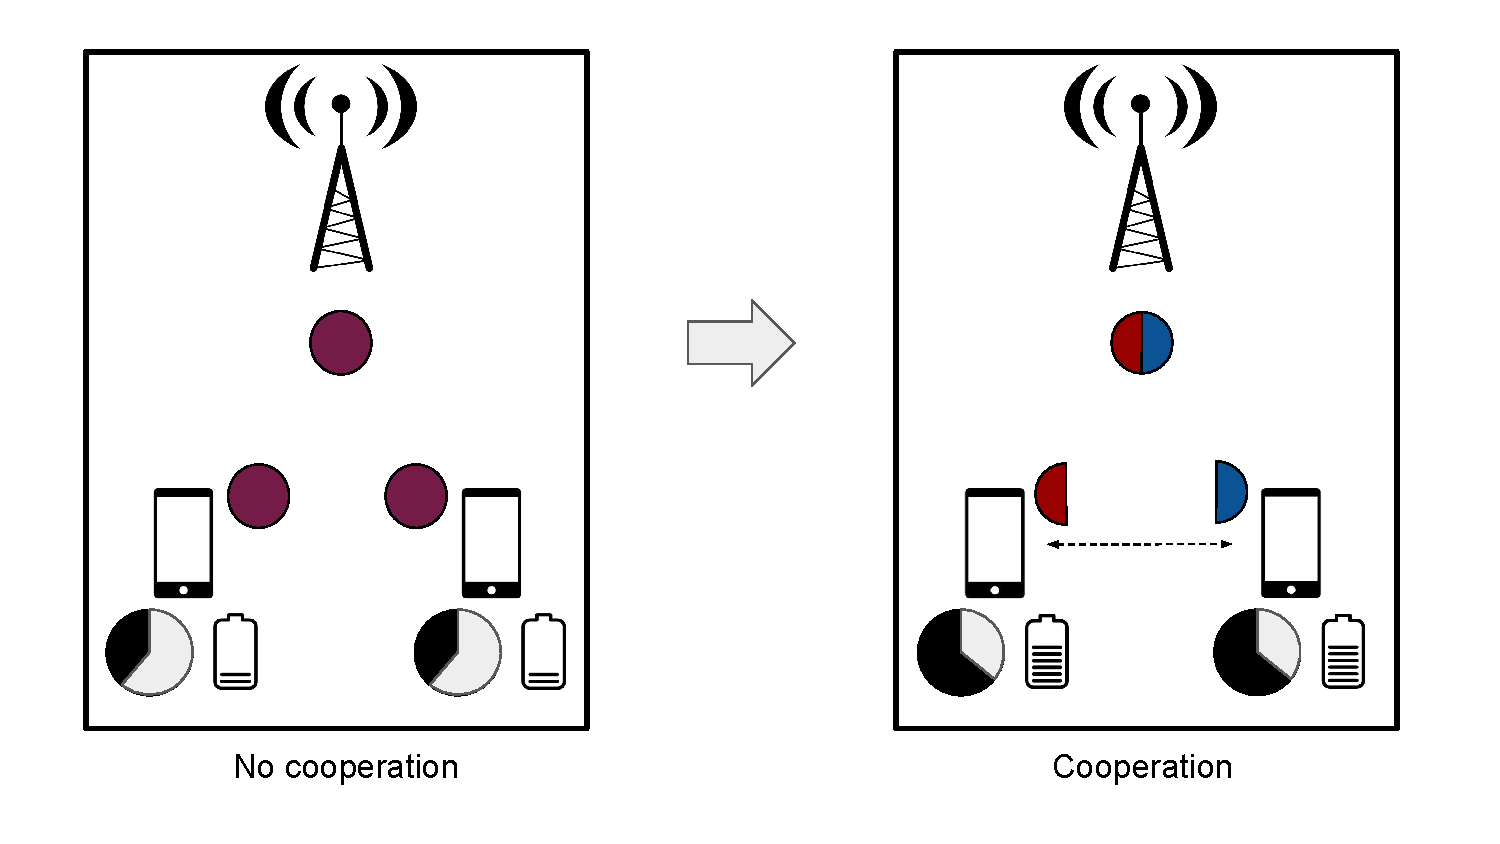
\includegraphics[width=\textwidth]{introduction/figures/cooperation.pdf}
  \caption{Cooperation in Wireless Networks.}
\label{fig:cooperation}
\end{figure}

Without cooperation, a purple content is sent to two mobile devices in a broadcast fashion. This incurs in posible a large downloading time to ensure both devices are satisfied reducing the throughput and increasing the energy consumption.  When cooperation is considered, the content now is split into smaller blue and red pieces where each of them is sent rapidly to each device. Then, the devices exploit short-range communications (dashed line) by exchanging their missing pieces. The key underlying idea is for the devices share their missing information through a faster, short-distance and reliable link which increases the total throughput and reduces the overal energy consumption. From an operator perspective, the information \textit{as a whole} is quickly disseminated into the receivers helping the \ac{BS} to offload data. At the end, the goal of reducing the use communication resources is achieved. In this way, mobile clouds allow to improve the overall network performance and user experience.

\subsection{Device to Device Communications in Mobile Networks}
\label{sec:d2d}
One of the key aspects to achieve the gains proposed by the cooperative approach is the short-range technology to be considered and its parameters to guarantee a fast and reliable link. Besides \ac{WLAN} technologies like \ac{WiFi}, there has been a large interest in \ac{D2D} communications \cite{lin2013comprehensive,asadi2014survey,feng2014device,tehrani2014device}. This permits the devices to share data without going through the \ac{BS} network which keeps the idea of data offloading. The work in \cite{asadi2014survey} proposes a classification of \ac{D2D} communications.

First, according to its spectrum use, the communications could be in the cellular network (inband) or outside in a local network (outband). Second, for inband \ac{D2D} the communications could take place in the spectrum of other mobile users (underlay) or another dedicated only to \ac{D2D} (overlay). Second, for outband \ac{D2D}, the coordination between cellular and local network radio interfaces is either controlled by the cellular \ac{BS} (controlled) or the users themselves (autonomous).

For network assisted or inband \ac{D2D}, authors in \cite{fodor2014design} review the key challenges to enable \ac{D2D} services. Device discovery, communication resource allocation and coordination for these type of communications are handled by the cellular network. Furthermore, \ac{D2D} based \ac{ProSe} have been included in \cite{3gpp2012prose} to use them in \ac{LTE-A} networks for an improved \ac{QoE}.

\subsection{Erasure Correcting Codes for Multicast Networks}
\label{sec:erasure_codes}
Another aspect that is relevant for cooperation gains in multicast scenarios is channel coding. The dynamics of the wireless medium, propagation conditions, noise and interference may degradate the received \ac{SINR} thus making reception unfeasible for some period of time. In the case of packet networks, this leads to \textit{erasure} channels where packets are either correctly received or lost. Therefore, to protect against packet erasures, some redundancy is added through channel coding with a \ac{FEC} technique also called an erasure correcting code. These techniques are relevant to make multicast applications reliable since feedback control through \ac{ACK} packets is not possible for a large number of devices.

Different erasure correcting codes might be used for reliable multicast applications. In the literature, we can find linear block codes such as \ac{RS} \cite{reed1960polynomial} or \ac{LDPC} \cite{gallager1962low}. More recently, \ac{LT} codes \cite{luby2002lt} and Raptor codes \cite{shokrollahi2006raptor} are codes that are more adaptable to the channel conditions than block codes. These latter type of codes are characterized by being: (i) Able to generate a very large number of coded symbols, i.e. rateless, (ii) close-to-optimal, i.e requiring a slightly higher amount of encoded symbols than the original set to decode and (iii) able to decode with a subset of coded symbols as long as there are no inter-dependencies in it. These erasure correction properties among others have led to consider Raptor codes for its standardization in multicast \ac{LTE-A} networks through the \ac{eMBMS} protocol \cite{embms2014general}.

Although these coding techniques are useful for multicast networks, they pose two major restrictions to apply them with the cooperative approach. First, this type of coding is made on a \textit{link} basis, meaning that for each hop encoding and decoding needs to take place. The required code processing for each hop brings delays and energy consumption due to computational aspects \cite{toemoeskoezi2015packet}. Second, as a consequence of the previous, these codes are not composable in principle. This implies that there are no known forms to create new coded packets from packets that have been coded previously without decoding in the case of rateless codes. Because of these limitations state of the art rateless codes are not ideal erasure correcting codes for cooperative wireless networks with \ac{D2D} due to the inherent processing in multihop.

\subsection{Random Linear Network Coding}
\label{sec:nc_rlnc}
% Network Coding, inter-session (XOR) and intra-session (RLNC)
Introduced by Alshwede et al. \cite{ahlswede2000network}, \ac{NC} appeared as an effective technology to remove the limitations presented previously. In this work, the authors presented a new paradigm shift for conveying information in communication networks. Instead of treating the packets as atomic, unmodifiable units at the intermediates node in a network, they are regarded as algebraic elements in a \ac{GF} that can be operated on to create new coded packets. In \cite{ahlswede2000network}, the authors considered the binary field to perform the algebraic operations. This type of coding became known later as inter-session network coding since packets from two sessions where mixed in the coding process. Due to the binary field nature, it also became known as XOR coding since this operation is congruent with the modulo-2 addition. However, limitation for this coding scheme is that specific topologies needs to occur for taking advantage of the codes which might not be the case in our scenarios.

Besides inter-session network coding, intra-session network coding known as \ac{RLNC} \cite{ho2006random}, was introduced by Ho et al. Here, coded packets are algebraic linear combinations of original set of packets from a single data flow. This permits to remove the limitation of sending \textit{particular} packets by now sending coded packets as linear equations of the originals. Given that packets are mixed from a single flow, there are no requirements for a specific topology to use \ac{RLNC}. This type of coding can made across any node in the network. Further, \ac{RLNC} is proven to achieve the multicast capacity from a flow perspective with very high probability \cite{koetter2003algebraic,ho2006random}. In this way, instead of typically encoding and decoding on a hop basis, coding is made on a \textit{network} basis. Relaying nodes can recode packets to reduce delay and still take advantage of the data representation for the next hop. In this sense, \ac{RLNC} appears as the only coding technique that overcomes the restrictions mentioned earlier in Section~\ref{sec:erasure_codes}.

\begin{figure}[h]
  \centering
  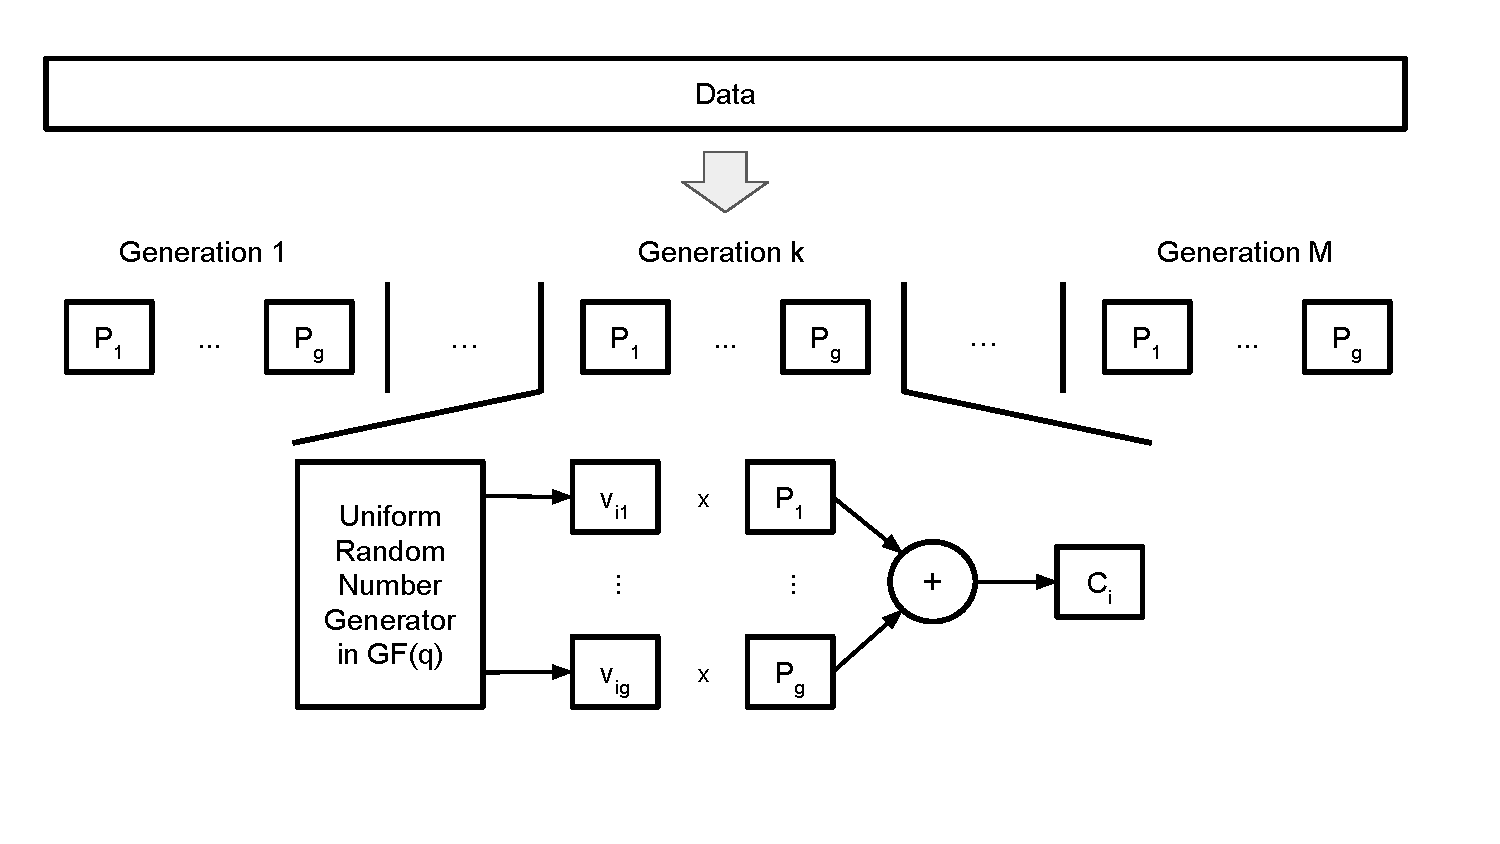
\includegraphics[width=\textwidth]{introduction/figures/RLNC.pdf}
  \caption{RLNC encoding process.}
\label{fig:rlnc_enc}
\end{figure}

As seen in Fig.~\ref{fig:rlnc_enc}, in \ac{RLNC} the information to be transmitted is split into packets which are grouped into sets called \textit{generations} \cite{chou2003practical}. Each generation $k = 1, \ldots, M$ consists of $g$ original packets $P_i,\ i = 1, \ldots, g$ used to create new coded packets as with any \ac{FEC} technique from Section~\ref{sec:erasure_codes}. For each generation, each coded packet generated is a linear combination of all the original packets $C_i = \sum_{j = 1}^g v_{ij} P_i,\ i \geq 1$. Here, $v_{ij}$ is the coding coefficient that multiplies packet $j$ in the process of creating packet $i$. The coefficients are picked uniformly at random from $GF(q)$ where $q$ is the field size. All the operations are properly defined under the arithmetics of $GF(q)$.

After creating a coded packet, it is necessary to signal the coding coefficients utilized for encoding to the decoder. The signalling method that guarantees potential recoding without major caveats, is to append each coding coefficient used to create that coded packet as overhead. For each coded packet there is an overhead of $|v_{ij}| = \sum_{j = 1}^g \log_{2}(q) = g \times \log_{2}(q),\ \forall i,j$ bits. To get the original packets, a decoder only needs to collect \textit{any} set of $g$ linearly independent coded packets to create a $g \times g$ matrix with the coding coefficients and perform Gaussian elimination \cite{fragouli2006network} to solve the linear equations made in the encoding process.

Despite being a relatively recent technology, practical applications of \ac{RLNC} started to appear a few years after its inception. The work of Chachulski et al. in \cite{chachulski2007more} considered \ac{MORE}, the first protocol using \ac{RLNC} which showed different achievable gains in real wireless mesh networks. Different potential \ac{RLNC} use cases can also be found in \cite{fragouli2006network}. For reliable multicast, various works have been made to quantify the gains of \ac{RLNC} against other transmission schemes in terms of erasure codes or policies. Among these, it can be mentioned: (i) throughput and delay gains of reliable multicast with \ac{RLNC} \cite{eryilmaz2008delay} and (ii) resource allocation of multicast \ac{RLNC} based networks \cite{chiti2013optimized,tassi2015resource} among others. Nevertheless, neither of these works consider cooperation or multicast \ac{D2D} communications. 

\subsection{RLNC for Multicast D2D Cooperative Networks}

Different from other erasure correcting codes, \ac{RLNC} is well-suited for multicast \ac{D2D} cooperative networks due to its recoding capability.

There has been different studies that addressed the impact of \ac{RLNC} code parameters, i.e. the generation size $g$ and the field size $q$, in both theoretical and practical applications with mobile devices\cite{heide2009network,lucani2009random,heide2011code,paramanathan2013lean}. According to them, there has major finding about the impact of the code parameters in its performance. For the field size, its effects are resumed in Table~\ref{tab:rlnc_parameters} for the case of a single encoder and decoder excluding packet erasures.

\begin{table}[h]
  \centering
  \caption{Field size effects in the code performance for one source-destionation with no erasures.}
  \begin{tabular}{|M{0.75cm}|M{2cm}|M{1.5cm}|M{2.65cm}|M{2cm}|}

    \hline
    $q$         & Linear Dependency & Signalling & Overhead Major Contributor & Field Complexity  \\
    \hline
    \hline
    $< 2^8$     & High       & Low        & Linear Dependency & Low \\
    \hline
    $\geq 2^8$  & Low        & High       & Signalling & High \\
    \hline

  \end{tabular}

\vspace{0.2cm}
\label{tab:rlnc_parameters}
\end{table}

Table~\ref{tab:rlnc_parameters} shows the effects of the field size for two principal regions: low and high field sizes. The criteria to separate them has been to consider a field size as high for values higher than $2^8$ for reasons that will be explained below. The table also displays various metrics to evaluate the performance of the code.

Linear dependency refers to the amount of linearly dependent coded packets that are generated during the transmission process. As more linearly independent coded packets are received during the transmission process, linearly dependent coded packets are generated more frequently towards the end of the transmission. Dependent packets are useless since they provide no new information to the decoder and are discarded. Once $g - 1$ independent coded packets have been received, the probability of generating a dependent coded packet is $\frac{1}{q}$ \cite{lucani2009random,heide2011code}. For the binary field, i.e. $GF(2)$, there is a 50\% probability of generating useless packets. In the case of $GF(2^8)$, this probability reduces to less than 0.5\% making it depreciable in practice. In terms of the generation size, the linear dependency effect can be observed on the average amount of transmissions for decoding. For $GF(2)$, $g + 1.667$ transmissions are required to decode the original set, whereas for $GF(2^8)$ it can be approximated to $g$ for practical purposes. 

Signalling is interpreted as the amount of bits required to represent the coding coefficients. These bits are attached to each coded packet and for each original packet. We referred to this value previously as $|v_{ij}| = |v| = g \times \log_{2}(q)$ which grows linearly with $g$ and logarithmically with $q$. For $GF(2)$, only 1 bit per packet is required to be included in each coded packet to signal the coding coefficients. However, for fields such as $GF(2^8)$ or higher, more than one byte is necessary for each original packet to signal its coding coefficients. Therefore for high generation sizes, high fields could potentially make the amount signalling even higher than the original packet size.

Thus, overhead accounts for both effects of the linear dependency and coding coefficients signalling respect to useful data. In Table~\ref{tab:rlnc_parameters}, it has been specified which is the effect that accounts for most of the total overhead in the specified region. For low fields, most of the overhead comes from linear dependency effect , but for higher field sizes the signalling from the coding coefficients becomes critical. 

%\cite{heide2012green,fitzek2013implementation,militano2014wi}

\todo{Make better table intro? Talk about cluster sizes?}

\subsection{Thesis Objectives}
Based in the previous background, this thesis considers to push the state of the art by using multicast \ac{D2D} mobile clouds in cooperative wireless networks with \ac{RLNC} since current techniques focuses mostly in \ac{D2D} communications based in unicast pairs with either \ac{RLNC} or non-composable rateless codes. The objectives of this thesis are to:

\begin{enumerate}

\item Define the regions and conditions in terms of network and code parameters parameters where cooperation with \ac{RLNC} provides a better performance than broadcast with \ac{RLNC} in terms of data throughput and energy consumption at the mobile devices.

\item Propose and study code constructions that permit to avoid the \ac{RLNC} tradeoff from Section~\ref{sec:nc_rlnc} to achieve minimum total overhead. In this sense, the objective is to find codes that permit to retain the low coding coefficients overhead from a low field size, but also the low number of transmissions overhead from high fields.

\item Study the dominating regimes and ideal cloud sizes to observe if there exists ideal values for high system throughput and low energy consumption.

\item Study the effect of transmission policies under a \ac{WLAN} scenario. In this case, medium access mechanisms to avoid interference should be considered.
\end{enumerate}

\begin{figure}[h]
  \centering
  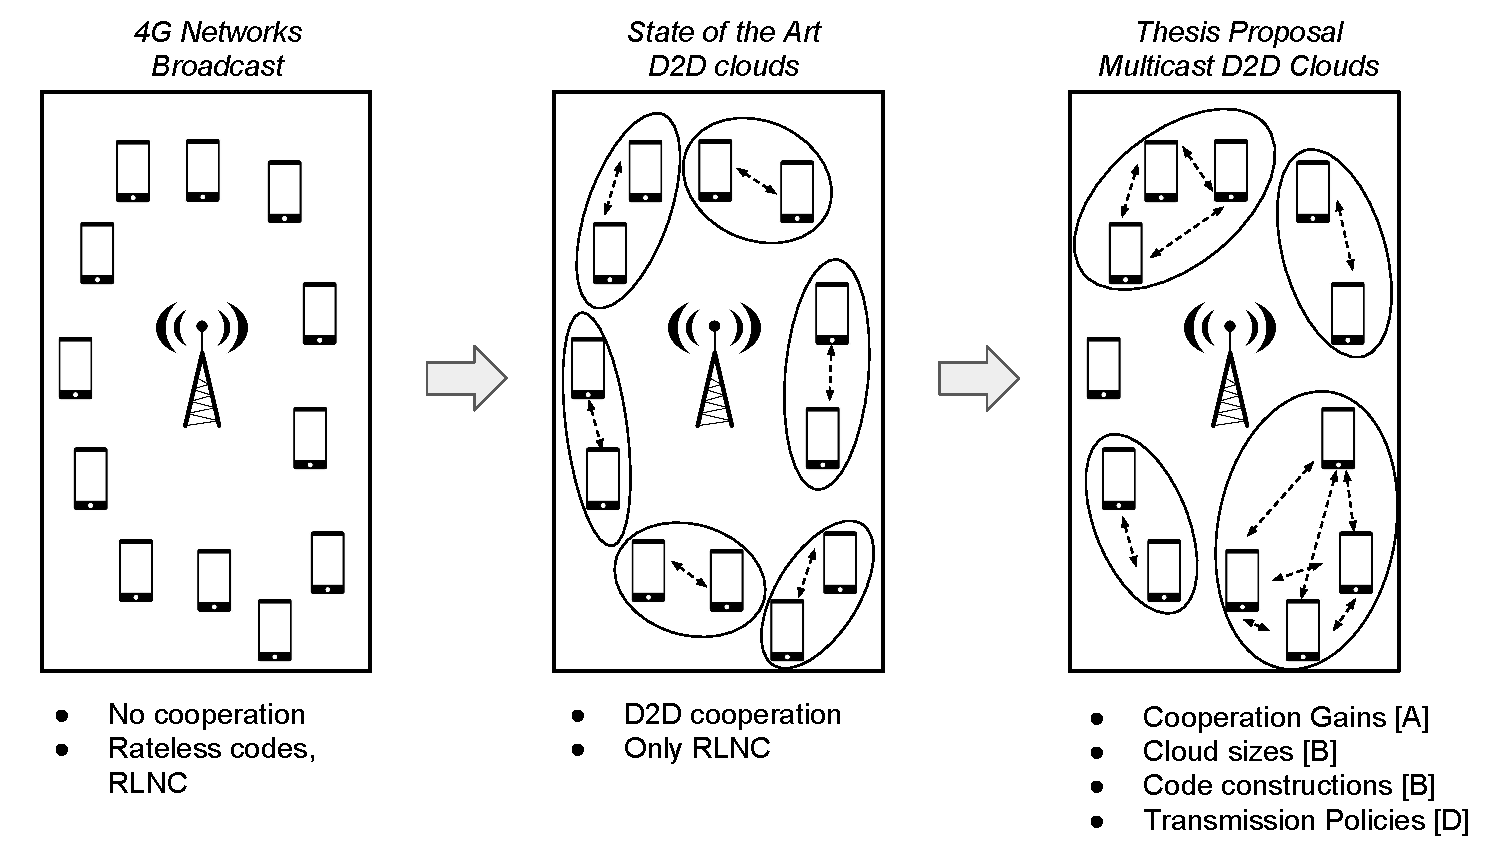
\includegraphics[width=\textwidth]{introduction/figures/thesis-diagrams.pdf}
  \caption{State of the Art and Thesis Proposal.}
\label{fig:proposal}
\end{figure}

From Fig.~\ref{fig:proposal}, the study for objective 1 was addressed in paper {[\ref{paper:paperA}]}. Objectives 2 and 3 were reviewed in paper {[\ref{paper:paperB}]}. Finally, objective 4 was addressed in paper {[\ref{paper:paperD}]} with a software tool implemented in paper {[\ref{paper:paperC}]} that uses Kodo and the open-source ns-3 simulator \cite{ns3link}.

\clearpage
%In principle, adding more users to the cloud enhances the realibility of it and minimizes the transmissions from the \ac{BS}. Still, this might increment the transmissions inside the clouds since .
